\definecolor{bostonuniversityred}{rgb}{0.8, 0.0, 0.0}
\definecolor{seagreen}{rgb}{0.18, 0.55, 0.34}

\section{Redes de Interconexão}

\subsection{Introdução}

\begin{frame}{Redes de Interconexão}
    \begin{itemize}
        \item Um sistema paralelo deve prover um meio de comunicação entre seus processadores, essas são chamadas de \textbf{redes de interconexão}
        \bigskip
        \item Podem ser implementadas de duas maneiras:
        \medskip
        \begin{itemize}
            \item Meio compartilhado;
            \medskip
            \item Meio comutado.
        \end{itemize}
    \end{itemize}
\end{frame}

\subsection{Meio Compartilhado}

\begin{frame}{Meio Compartilhado}
    \begin{columns}
    \column{0.6\linewidth}
        \fontsize{10pt}{7.2}\selectfont
        \begin{itemize}
            \item Um processador envia a mensagem, todos recebem e somente os destinatários interpretam.
            \medskip
            \begin{itemize}
                \item \textbf{Ex}: Ethernet.
            \end{itemize}
            \bigskip
            \item Processadores esperam até que o meio esteja livre para enviar uma mensagem.
            \bigskip
            \item \textbf{Colisão}:
            \medskip
            \begin{itemize}
                \item Ambas mensagens são descartadas;
                \medskip
                \item Após um tempo aleatórios, os remetentes reenviam a mensagem;
                \medskip
                \item \textbf{{\color{bostonuniversityred}Leva a uma perda de performance do meio de comunicação.}}
            \end{itemize}
        \end{itemize}
        \fontsize{10pt}{7.2}\selectfont
        \column[b]{0.4\linewidth}
        \begin{figure}[H]
            \centering
            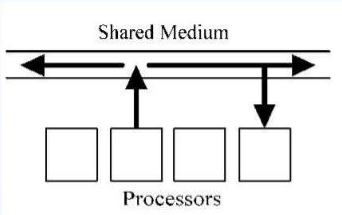
\includegraphics[width=1\linewidth]{img/redes_de_interconexao/shared}
            \caption{Rede compartilhada}
            \label{fig:shared}
        \end{figure}
    \end{columns}
\end{frame}

\subsection{Meio Comutado}

\begin{frame}{Meio Comutado}
    \begin{columns}
        \column{0.6\linewidth}
            \begin{itemize}
                \item Comunicação ponto-a-ponto entre par de processadores.
                \medskip
                \item Cada processador tem seu meio de comunicação individual para o comutador.
                \medskip
                \item {\color{seagreen}\textbf{Vantagens: Comunicação simultânea e escalabilidade.}}
            \end{itemize}
        \column{0.4\linewidth}
            \begin{figure}[H]
                \centering
                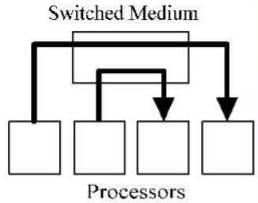
\includegraphics[width=1\linewidth]{img/redes_de_interconexao/switced}
                \caption{Rede comutada}
            \label{fig:sitced}
        \end{figure}
    \end{columns}
\end{frame}

\begin{frame}{Topologia em Redes de Comutação}
    \begin{itemize}
    \only<1>{ \item Topologias são representadas por grafos:
        \begin{itemize}
            \item \textbf{Nós:} Processadores ou comutadores.
            \medskip
            \item \textbf{Arestas:} Meios de comunicação entre os nós.
        \end{itemize}
    \bigskip
}
\only<2>{
    \item Como avaliar a eficiência de uma topologia:
    \medskip
    \begin{itemize}
    \item \textbf{Diâmetro:} Maior distância entre dois nós comutadores. Menor $\rightarrow$ Melhor, provê um limite inferior de complexidade para algoritmos paralelos
    \smallskip
    \item \textbf{Largura de Bisecção:} Número mínimo de arestas que precisam ser removidas para dividir a rede em duas metades. Maior $\rightarrow$ Melhor, provê um limite inferior de complexidade para algoritmos paralelos através da divisão da quantidade de dados que precisam ser transmitidos pela largura de bisecção.
    \smallskip
    \item \textbf{Arestas por nó comutador:} Melhor se a quantidade de arestas por nó comutador é independente do tamanho da rede, provendo escalabilidade.
    \smallskip
    \item \textbf{Comprimento constante de arestas:} Melhor se o comprimento das arestas é independente do tamanho da rede, provendo escalabilidade.
    \end{itemize}
}
    \end{itemize}
\end{frame}

\begin{frame}{Topologias em Redes de Comutação - Exemplos}
	\begin{itemize}
		\item \textbf{Redes 2-D \textit{Mesh}}
		\bigskip
		\begin{itemize}
			\item Grafo direcionado.
			\medskip
			\item Comunicação permitida somente entre vizinhos comutadores.
			\smallskip
			\begin{itemize}
				\item Algumas tem exceções: \textit{wraparound connections.}
			\end{itemize}
		\end{itemize}
	\end{itemize}
	\begin{columns}
		\column{0.75\linewidth}
		\hfill
		\begin{figure}[H]
			\centering
			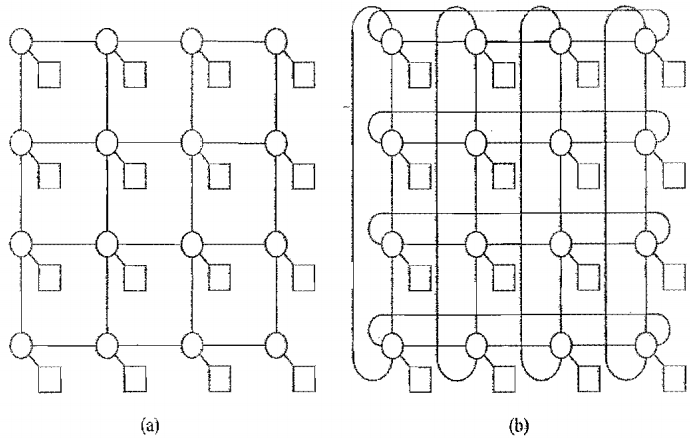
\includegraphics[width=.75\linewidth]{img/redes_de_interconexao/2D-mesh}
			\caption[(a) Rede 2-D mesh simples (b) Rede 2-D mesh com wraparound connections]{(a) Rede 2-D mesh simples (b) Rede 2-D mesh com \textit{wraparound connections}}
			\label{fig:2D-mesh}
		\end{figure}
		\column[b]{0.25\linewidth}
		\begin{itemize}
			\item \textbf{Círculos:} comutadores.
			\smallskip
			\item \textbf{Quadrados:} processadores.
		\end{itemize}
	\end{columns}
\end{frame}

\begin{frame}{Topologias em Redes de Comutação - Exemplos}
	\begin{itemize}
		\item \textbf{Hipercubo}
		\bigskip
		\begin{itemize}
			\item Grafo não direcionado.
			\medskip
			\item Dois nós comutadores são adjacentes se seus \textit{labels} diferem em um \textit{bit}.
		\end{itemize}
	\end{itemize}
	\begin{columns}
		\column{0.75\linewidth}
		\hfill
		\begin{figure}[H]
			\centering
			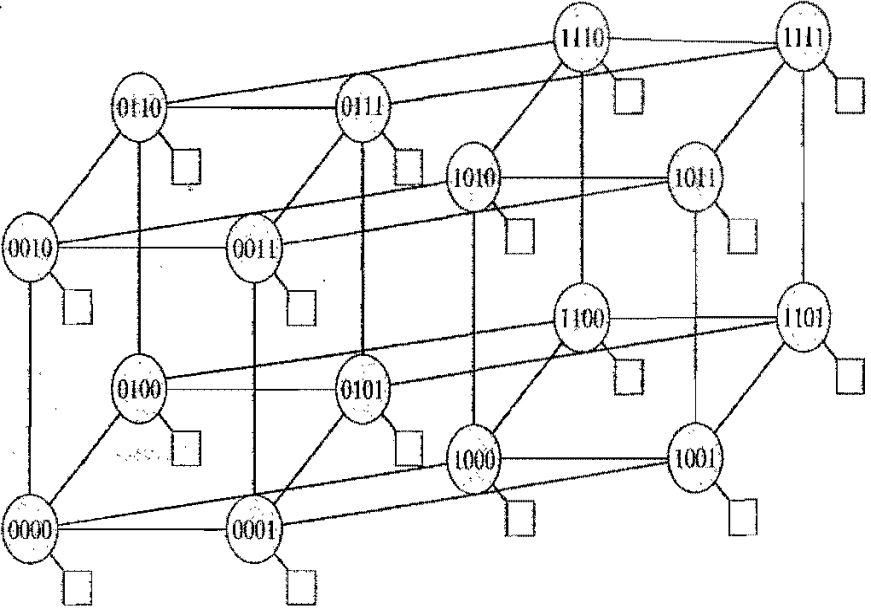
\includegraphics[width=.73\linewidth]{img/redes_de_interconexao/Hyper.png}
			\caption[Hypercubo 4-dimensional]{Hipercubo 4-dimensional}
			\label{fig:hyper}
		\end{figure}
		\column[b]{0.25\linewidth}
		\begin{itemize}
			\item \textbf{Círculos:} comutadores.
			\smallskip
			\item \textbf{Quadrados:} processadores.
		\end{itemize}
	\end{columns}
\end{frame}

\begin{frame}
\begin{center}
\begin{figure}[H]
\centering
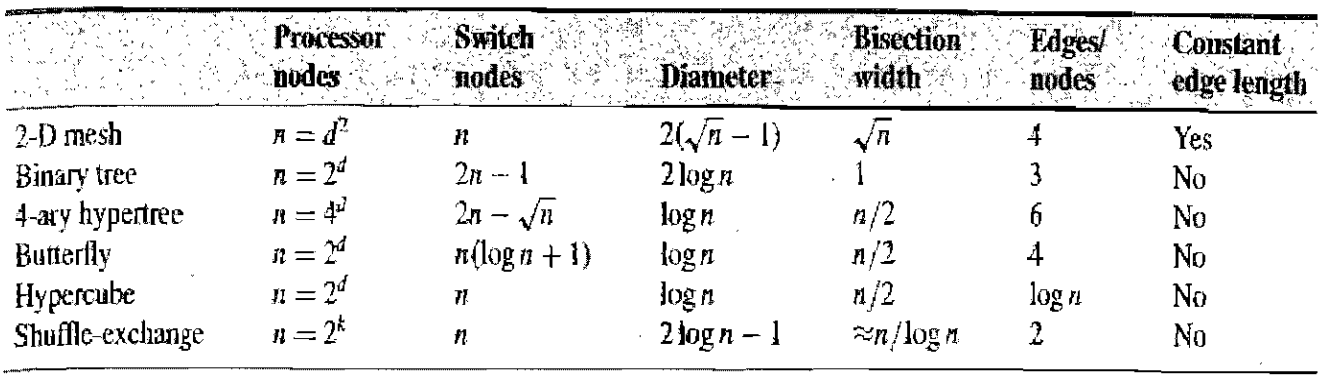
\includegraphics[width=1\linewidth]{img/redes_de_interconexao/compara}
\caption[Comparação entre diferentes topologias]{Comparação entre diferentes topologias}
\label{fig:compara}
\end{figure}
\end{center}

\end{frame}

